\begin{figure}[h!]
   \makebox[\textwidth]{%
      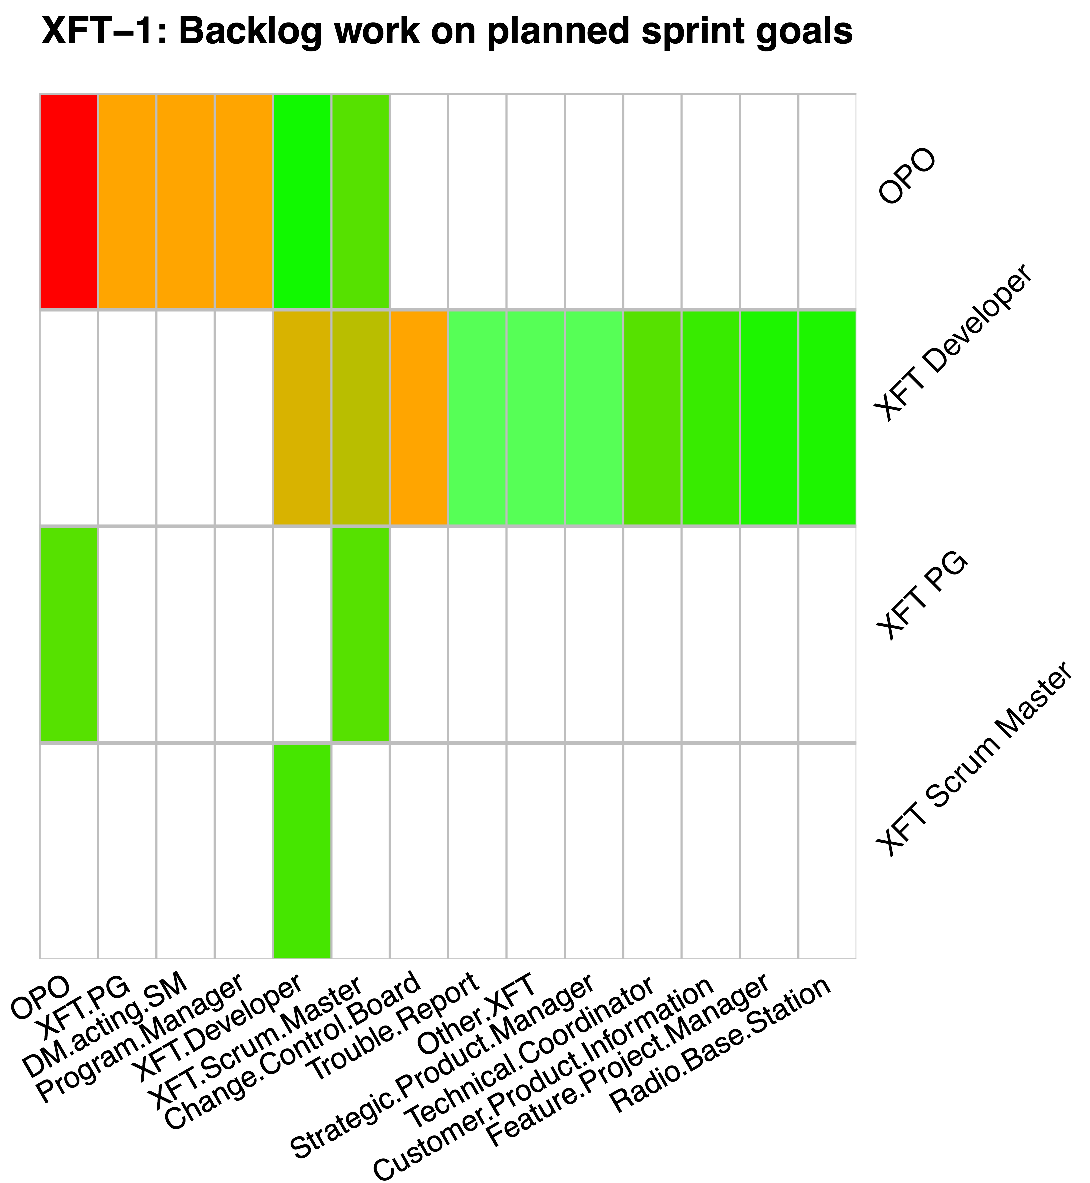
\includegraphics[width=0.49\textwidth]{figures/heatmaps/ms2-_b_.pdf}%
      \hfill    
      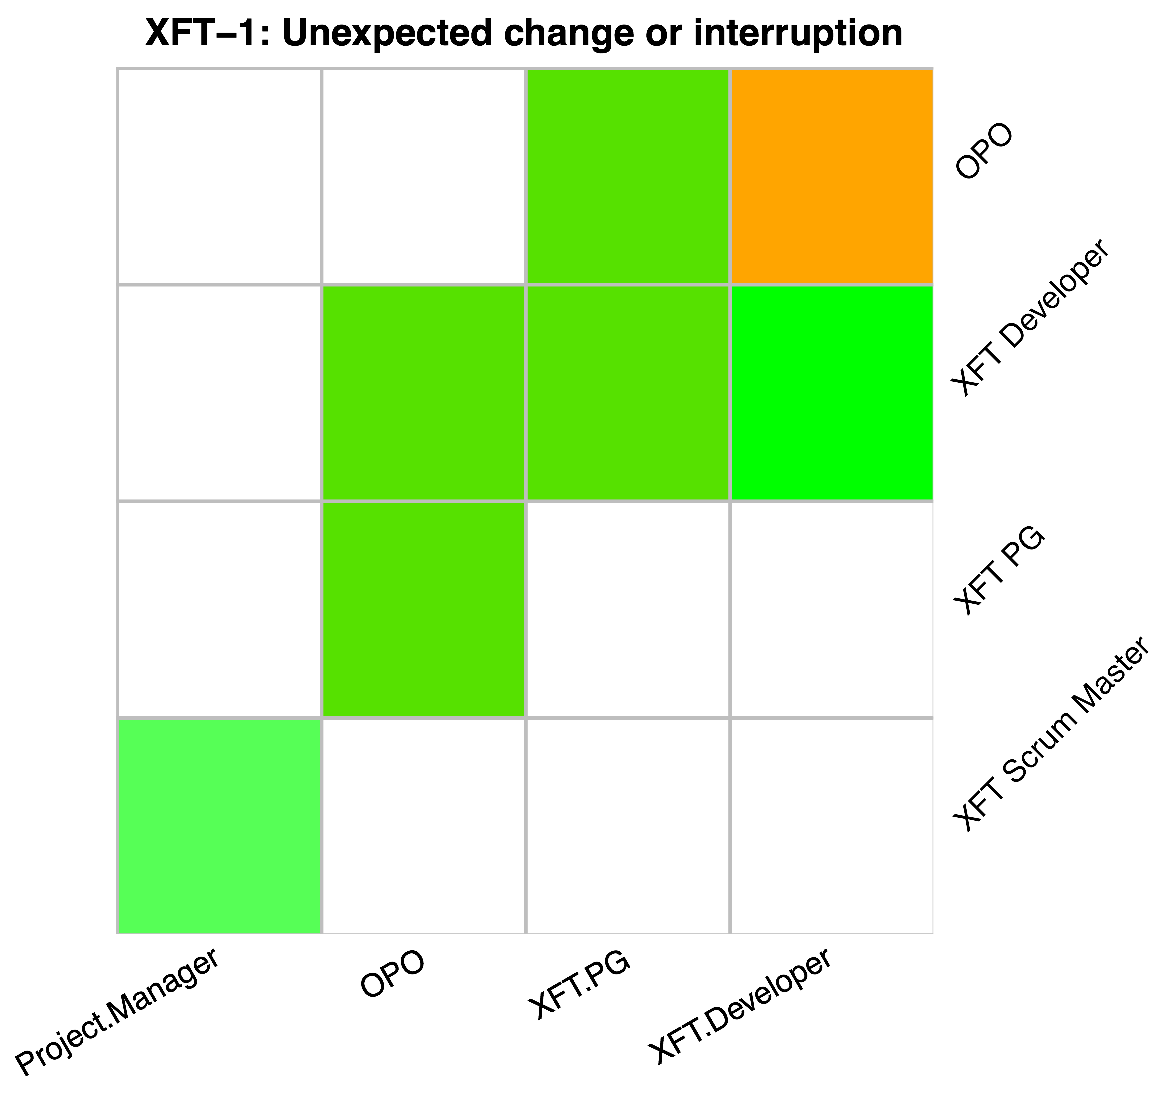
\includegraphics[width=0.49\textwidth]{figures/heatmaps/ms2-_u_.pdf}%
   }\\[0.5cm]% If you want some vertical space
   \makebox[\textwidth]{%
      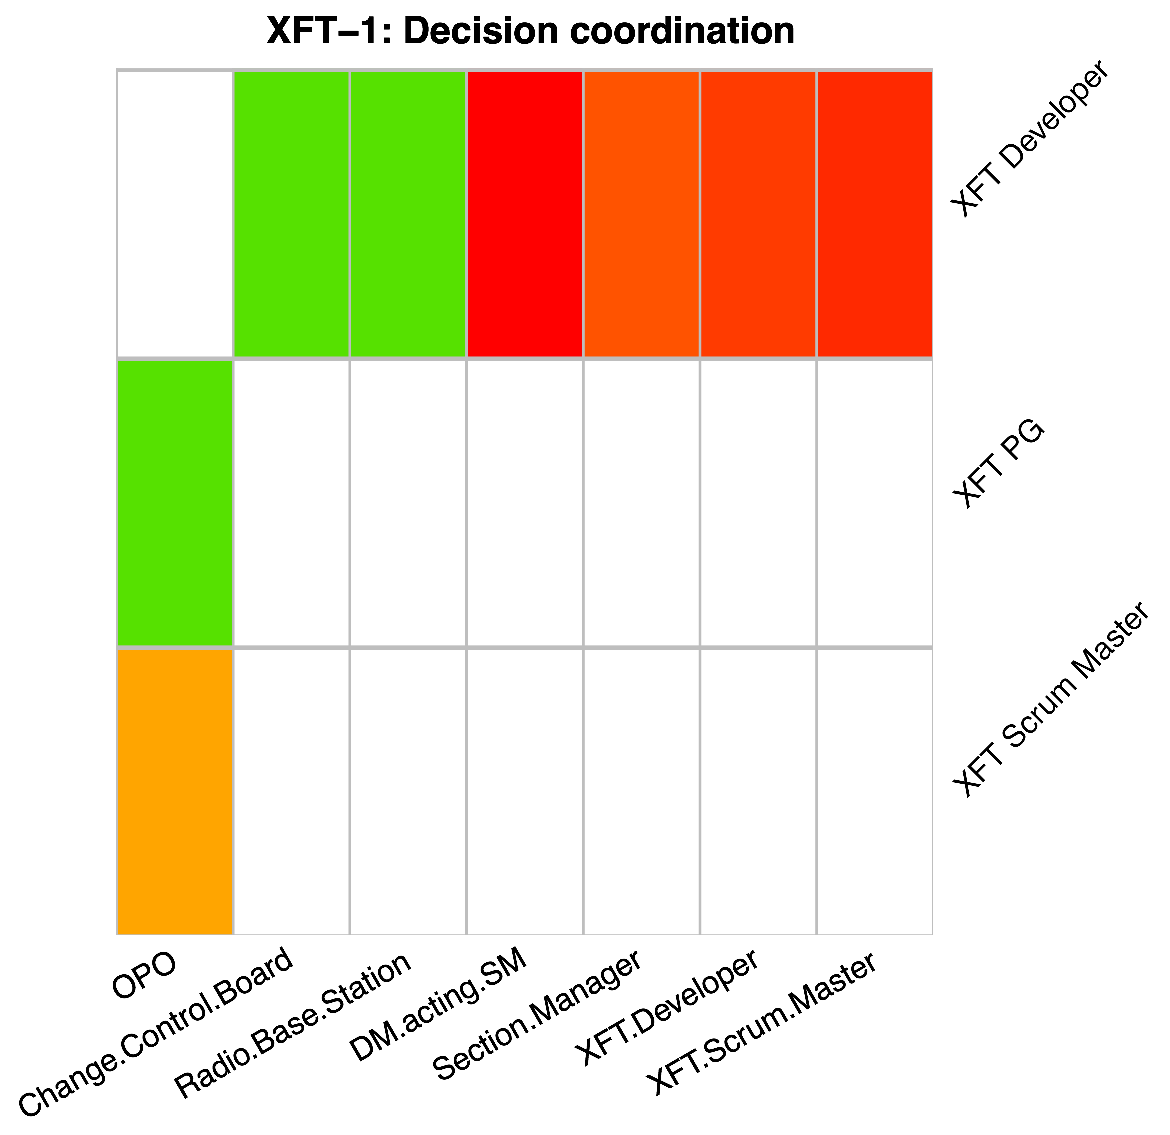
\includegraphics[width=0.49\textwidth]{figures/heatmaps/ms2-_d_.pdf}%
      \hfill    
      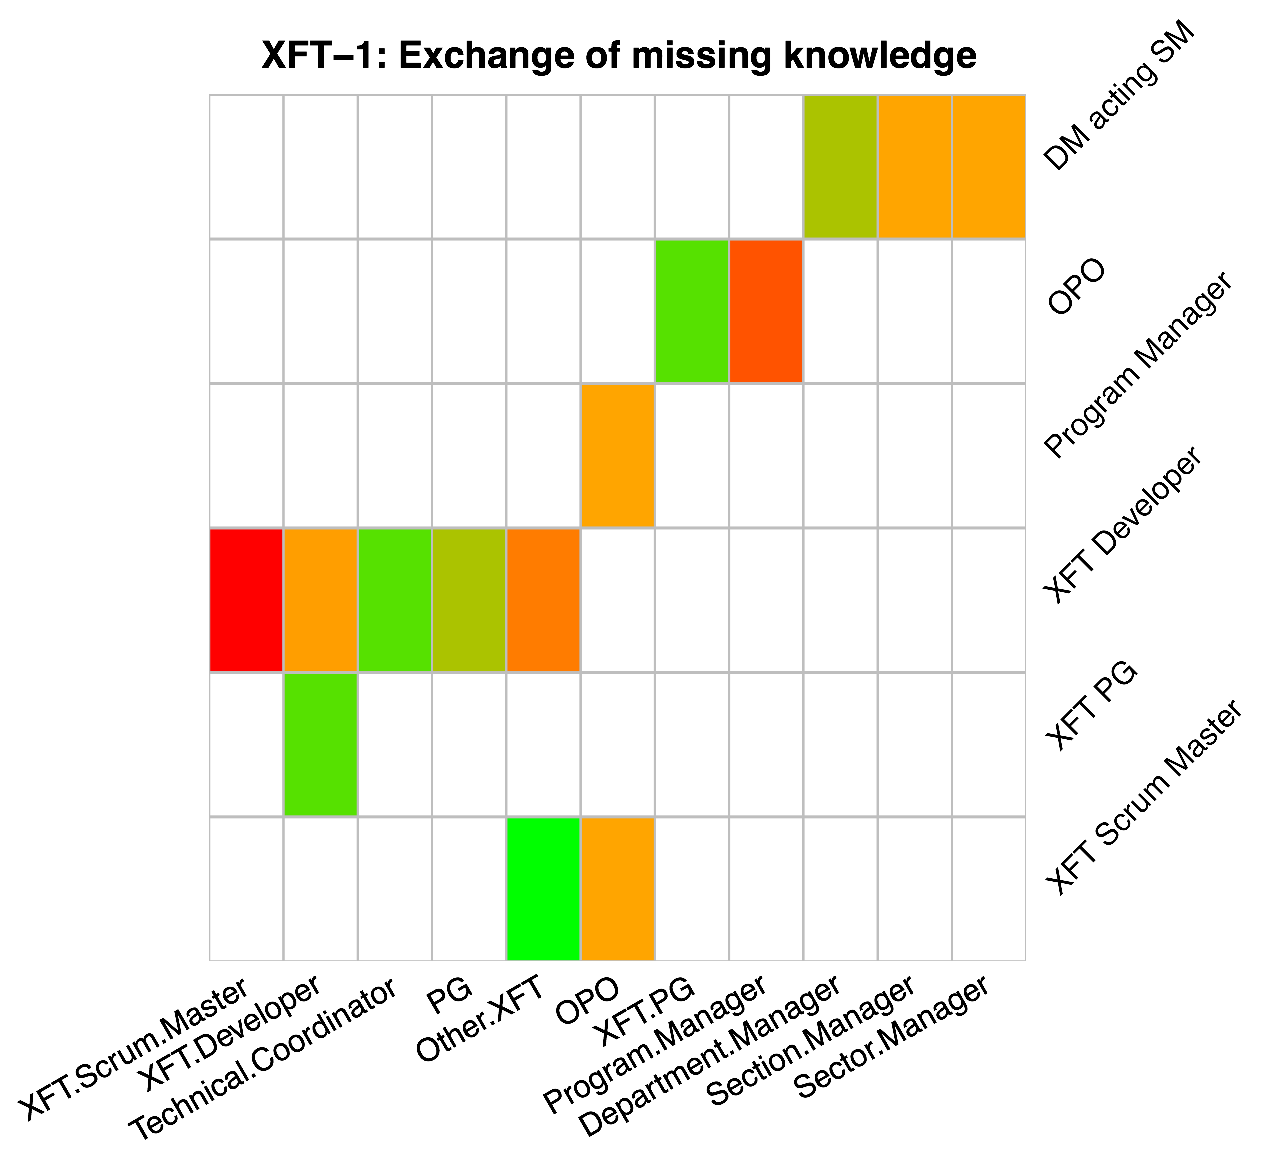
\includegraphics[width=0.49\textwidth]{figures/heatmaps/ms2-_e_.pdf}%
   }\\[0.5cm]% If you want some vertical space
   \makebox[\textwidth]{%
      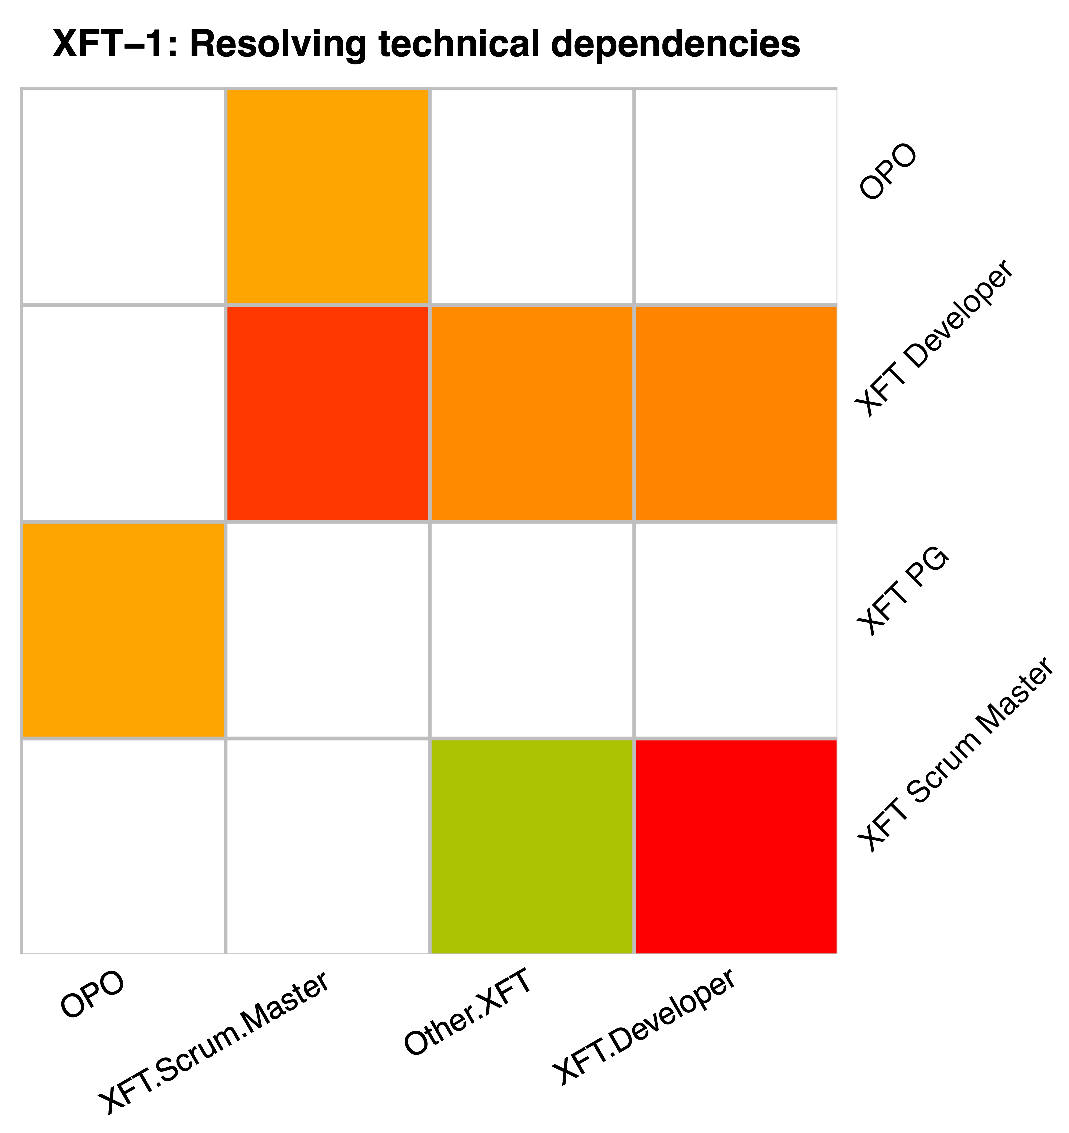
\includegraphics[width=0.49\textwidth]{figures/heatmaps/ms2-_r_.pdf}}
      \caption{XFT-1: Differences in intensities depending on communication nature}
      \label{fig:hm-overall-ms2
   }
\end{figure}

\begin{figure}[h!]
    \makebox[\textwidth]{%
        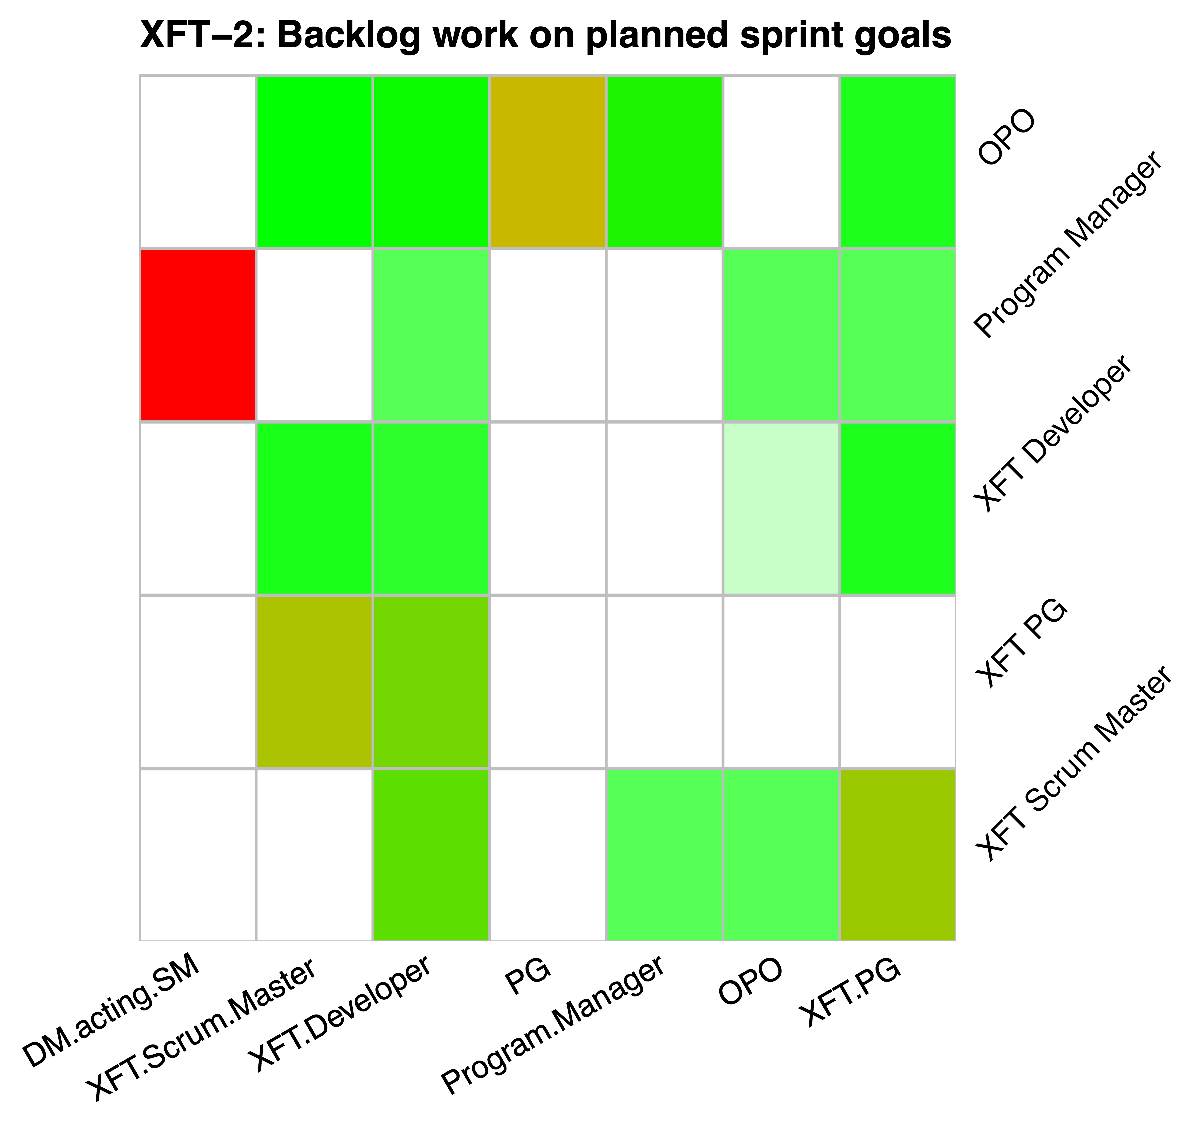
\includegraphics[width=0.49\textwidth]{figures/heatmaps/picnic-_b_.pdf}%
        \hfill    
        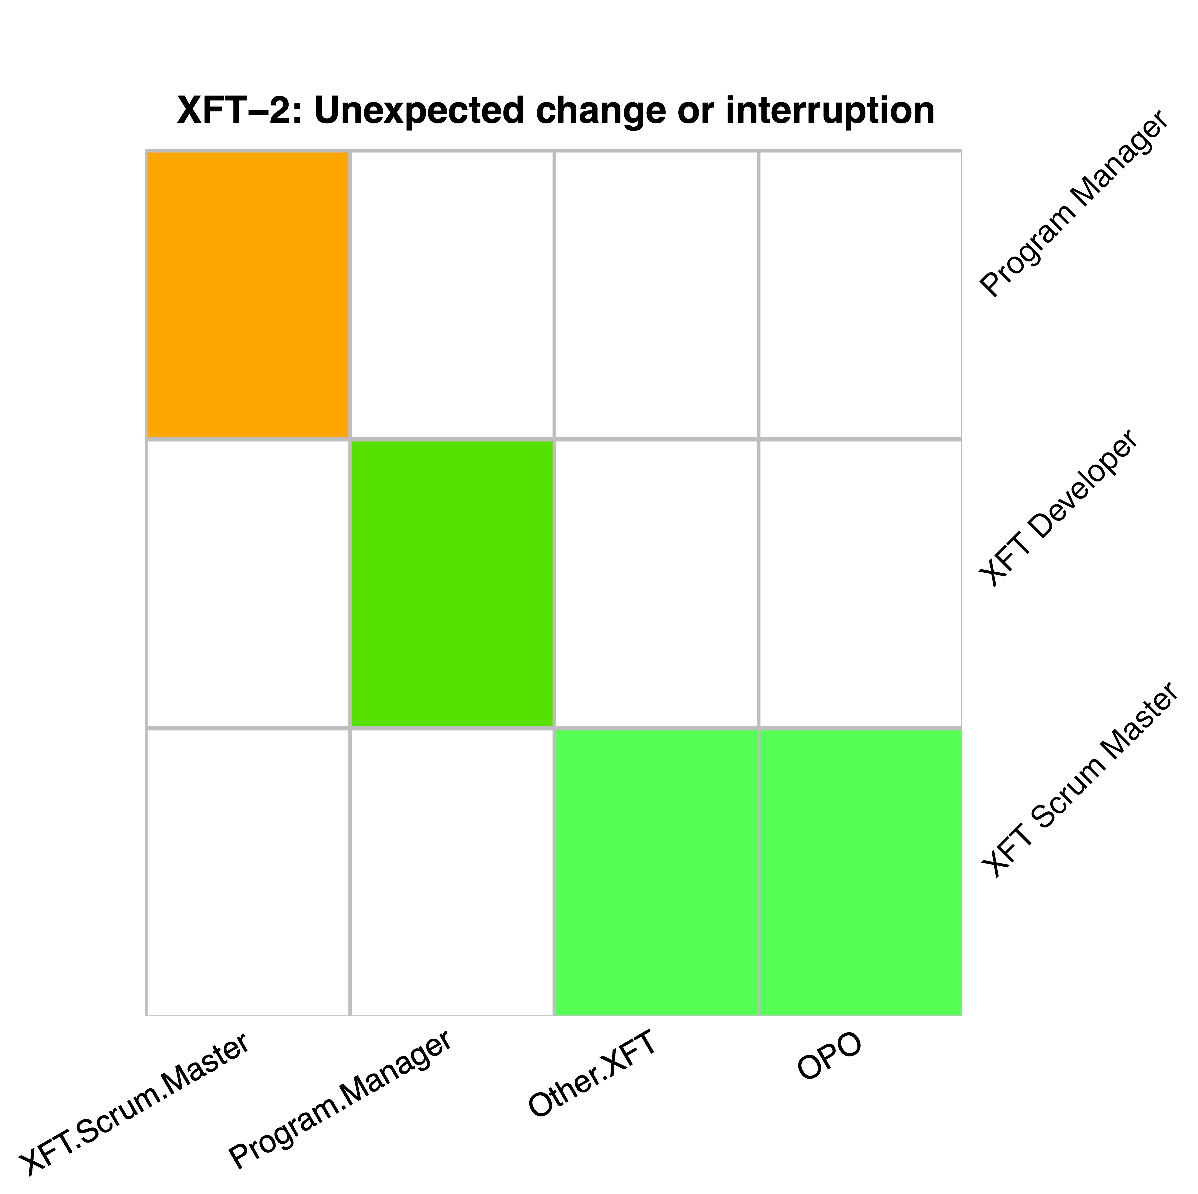
\includegraphics[width=0.49\textwidth]{figures/heatmaps/picnic-_u_.pdf}%
    }\\[0.5cm]% If you want some vertical space
    \makebox[\textwidth]{%
        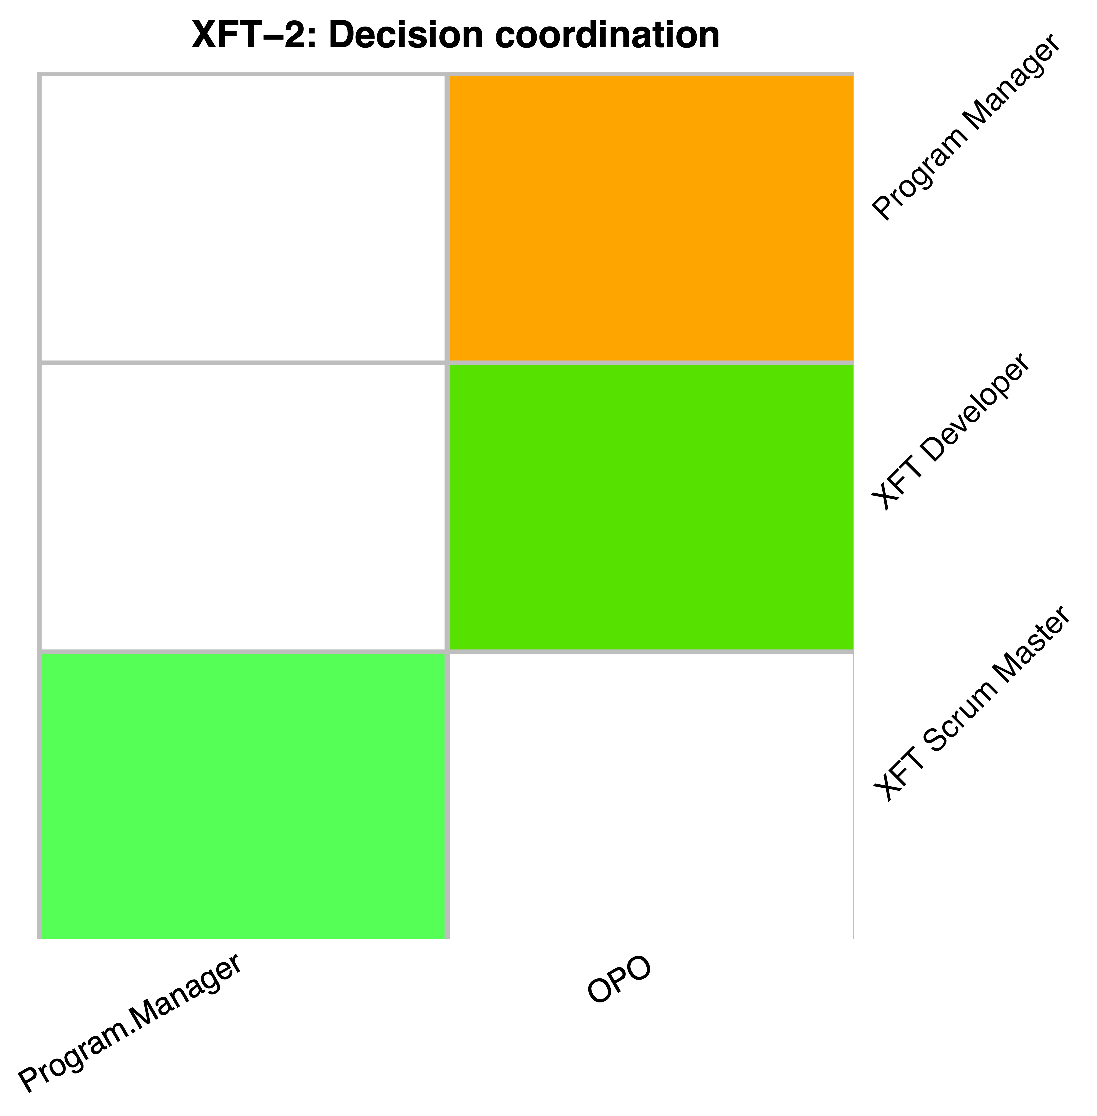
\includegraphics[width=0.49\textwidth]{figures/heatmaps/picnic-_d_.pdf}%
        \hfill    
        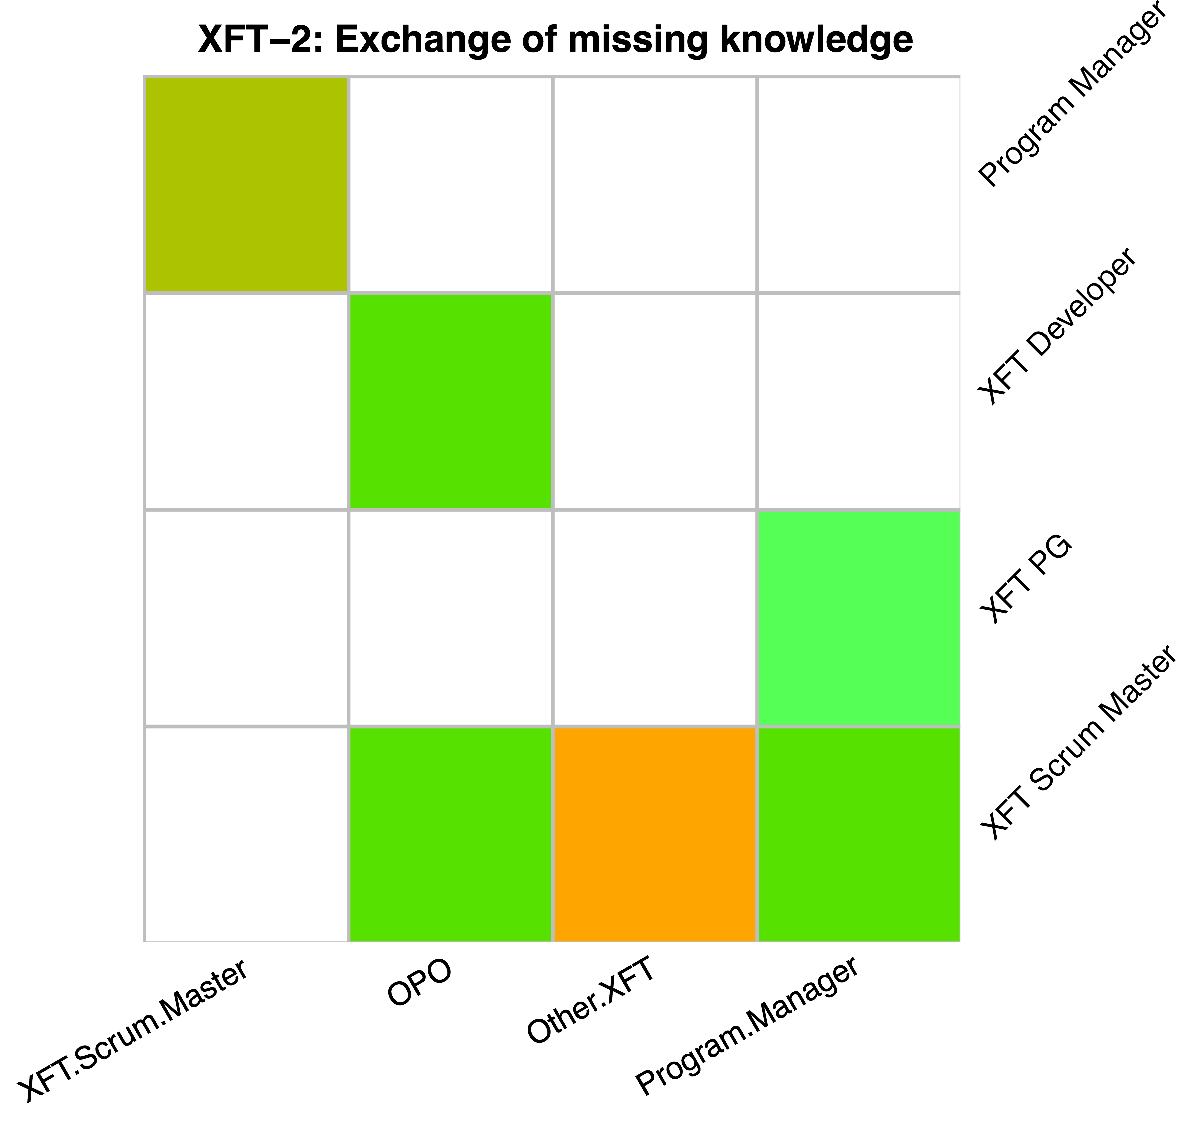
\includegraphics[width=0.49\textwidth]{figures/heatmaps/picnic-_e_.pdf}%
    }\\[0.5cm]% If you want some vertical space
    \makebox[\textwidth]{%
        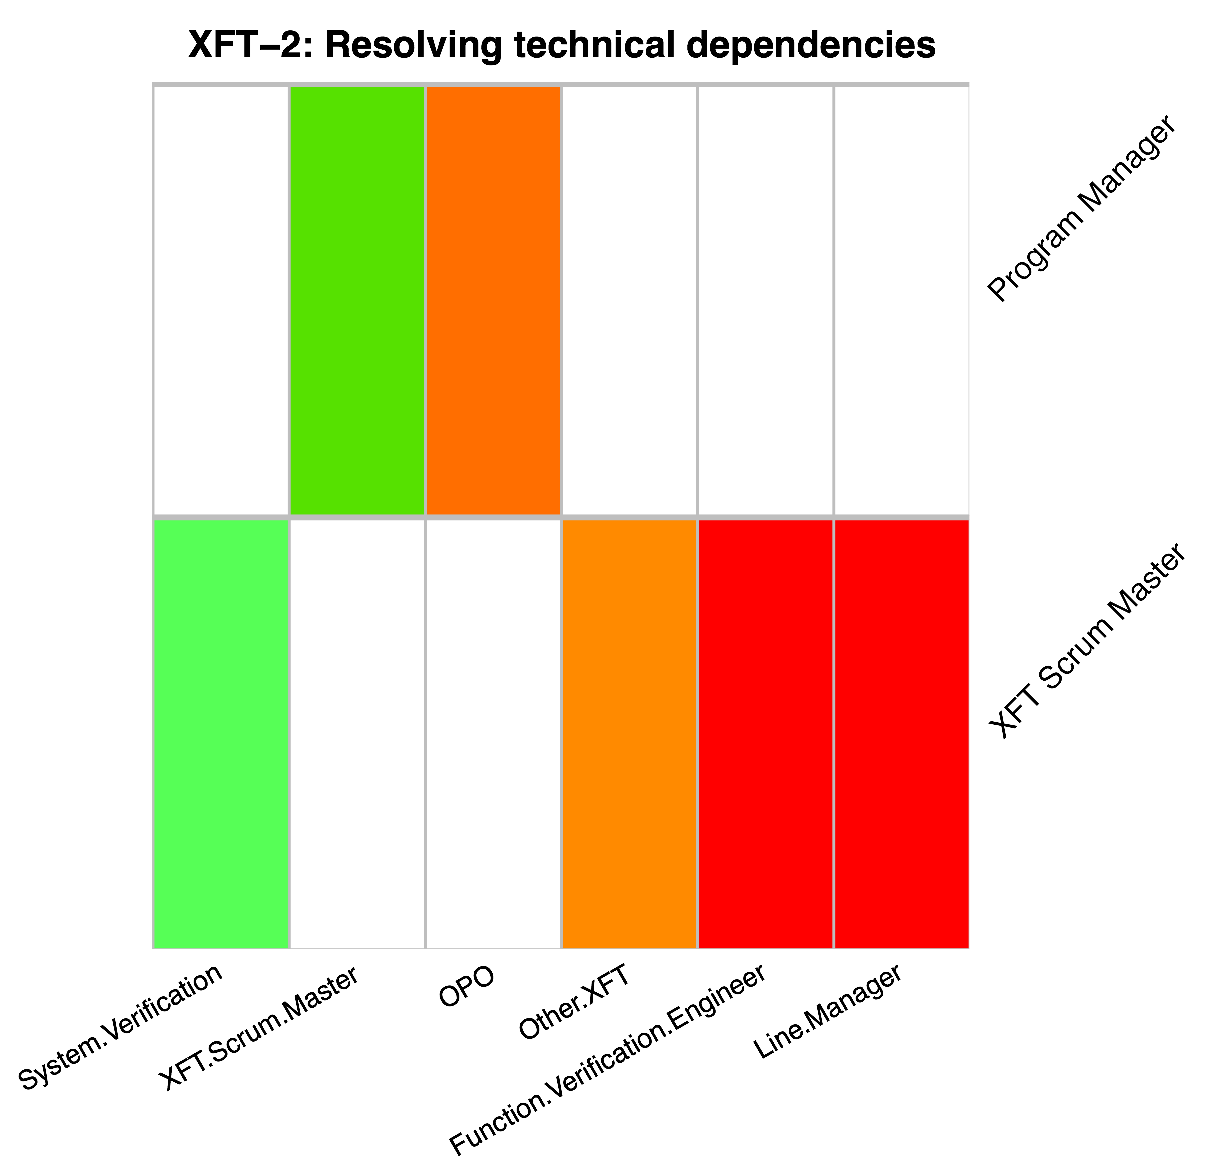
\includegraphics[width=0.49\textwidth]{figures/heatmaps/picnic-_r_.pdf}}
    \caption{XFT-2: Differences in intensities depending on communication nature}
    \label{fig:hm-overall-picnic}
\end{figure}